%\TODO{Introduction mentions interoperability between two OpenMP runtimes. But this section does not mention this. That is part of use case #2}

\subsection{Use Cases of OpenMP Interoperability}
We have identified four use cases of OpenMP interoperating with itself and other parallel programming models. 
\subsubsection{Interacting With User threads}
\textbf{Definition}
A user thread is a thread that is not created by OpenMP implementation. A user thread 
could become an OpenMP initial thread. 

The most common example of user threads are POSIX Threads, 
usually referred to as Pthreads with implementation available on most Unix-like 
POSIX-compliant systems. There are also implementations of other thread libraries, 
for example, Windows Native threads and language based threading support such as 
Java threads or others (e.g. qthreads). 

Figure~\ref{fig:pthread-omp} shows an example of having three user 
threads (two PThreads and one thread of the main program) in an OpenMP program. 
The two three threads execute in parallel after the two PThreads are created. 
Each thread calls a function that will enter into
OpenMP threading parallelism. So they all become OpenMP initial threads. How the 
user threads (PThreads in this example) interact with the OpenMP threading mechanisms
in the runtime is up to the implementation. They may share the same OpenMP runtime
instance or each has its own OpenMP runtime instance. 

\begin{figure}[t]
\centering
  \fbox{
 % \lstset{basicstyle=\ttfamily\scriptsize,language=c}
  \lstset{basicstyle=\ttfamily\scriptsize,language=c,numbers=left, %,frame=single,
  deletekeywords={int,if,else,while},
  morekeywords={pragma,omp,target,device,map,
  tofrom,to,from,alloc,parallel,shared,reduction,data,collapse,
  private,dist_iteration,match_range,halo,exchange},
  numbersep=12pt,numberstyle=\color{red}}
  \lstinputlisting{pthread-omp.c}

}
\caption{Three user threads (two Pthreads and one main thread) with OpenMP}
  \label{fig:pthread-omp}
\end{figure}

\subsection{Impacts and Discussions}
A user thread in a program adds additional level(s) in the overall ``threading''
hierarchy of a program. Those additional levels could be on top of OpenMP threading 
mechanism when a user thread becomes an OpenMP initial thread that creates OpenMP thread
parallelism, or beneath the OpenMP threading mechanism when an OpenMP thread spawns 
a user thread, or the the mix of both. In the example from Figure~\ref{fig:pthread-omp}, 
one can view this in a two-level threading parallelism: the top level user thread 
parallelism and the bottom level OpenMP threading parallelism.

These additional levels of threading increase the complexity of a program, both for 
users in the aspect of reasoning the parallel and synchronization behavior of a program, 
and also for the implementation and runtime system in terms of resource management and 
interactions. Adding to the complexity is the facts that a user thread may be created 
through a call to a library function whose paralelism (OpenMP) behavior is not known to 
the callee. Typical issues for example: 
\begin{itemize}
\item Does each user thread use the same OpenMP runtime libraries or not? 
	If not using the same library, how to handle symbol name 
	conflicts of two more different OpenMP runtime libraries. 
\item For user threads that use the same OpenMP runtime library, does the user threads each create its own runtime instance or they share one?
\item For user threads each of which has its own runtime instance (from the same or 
	different runtime library), how to coordinate the resource management among those
	runtime instances to address such issues as oversubscriptions and the affinity
	between user threads?
\end{itemize}

It is important to note that approaches to address those issues are very implementation
dependent, requiring protocol and agreement in the runtime behavior and/or interfaces 
of different OpenMP implementations. It may not be realistic to solve some of the issue
from the language standard, and should be left to users to deal with them. In this
aspect, we still hope this report could provide userful information and practices 
for users. 



\subsubsection{Interacting with Other OpenMP Programs}
Often a parallel machine is shared by users running multiple programs at the same time.
It is very likly that multiple OpenMP programs coexist within the same computation node. 
The OpenMP programs can be compiled by a same OpenMP compiler or different compilers. 
Current, an OpenMP implementation, including its runtime, assumes that it fully occupies the entire computation node,
without considering the possibility of existence of other running OpenMP programs and their supportive OpenMP runtime instances. 
The coexistence of multiple OpenMP runtime instances raises the following questions:
\begin{itemize}
\item How many OpenMP programs are running currently?
\item Which OpenMP runtime system is being used by a running OpenMP program?
\item What resources are used by each of them?
\item How do the concurrently executing OpenMP programs interact with each others to ensure optimal resource utilization?
\end{itemize}


\subsubsection{Interacting With Other Parallel Systems or Libraries}
It is now very common that an application uses multiple parallel libraries at the same time, which could be developed 
using OpenMP, TBB, Cilkplus, C++11, and other parallel libraries. 

\begin{figure}[h!]
  \centering
      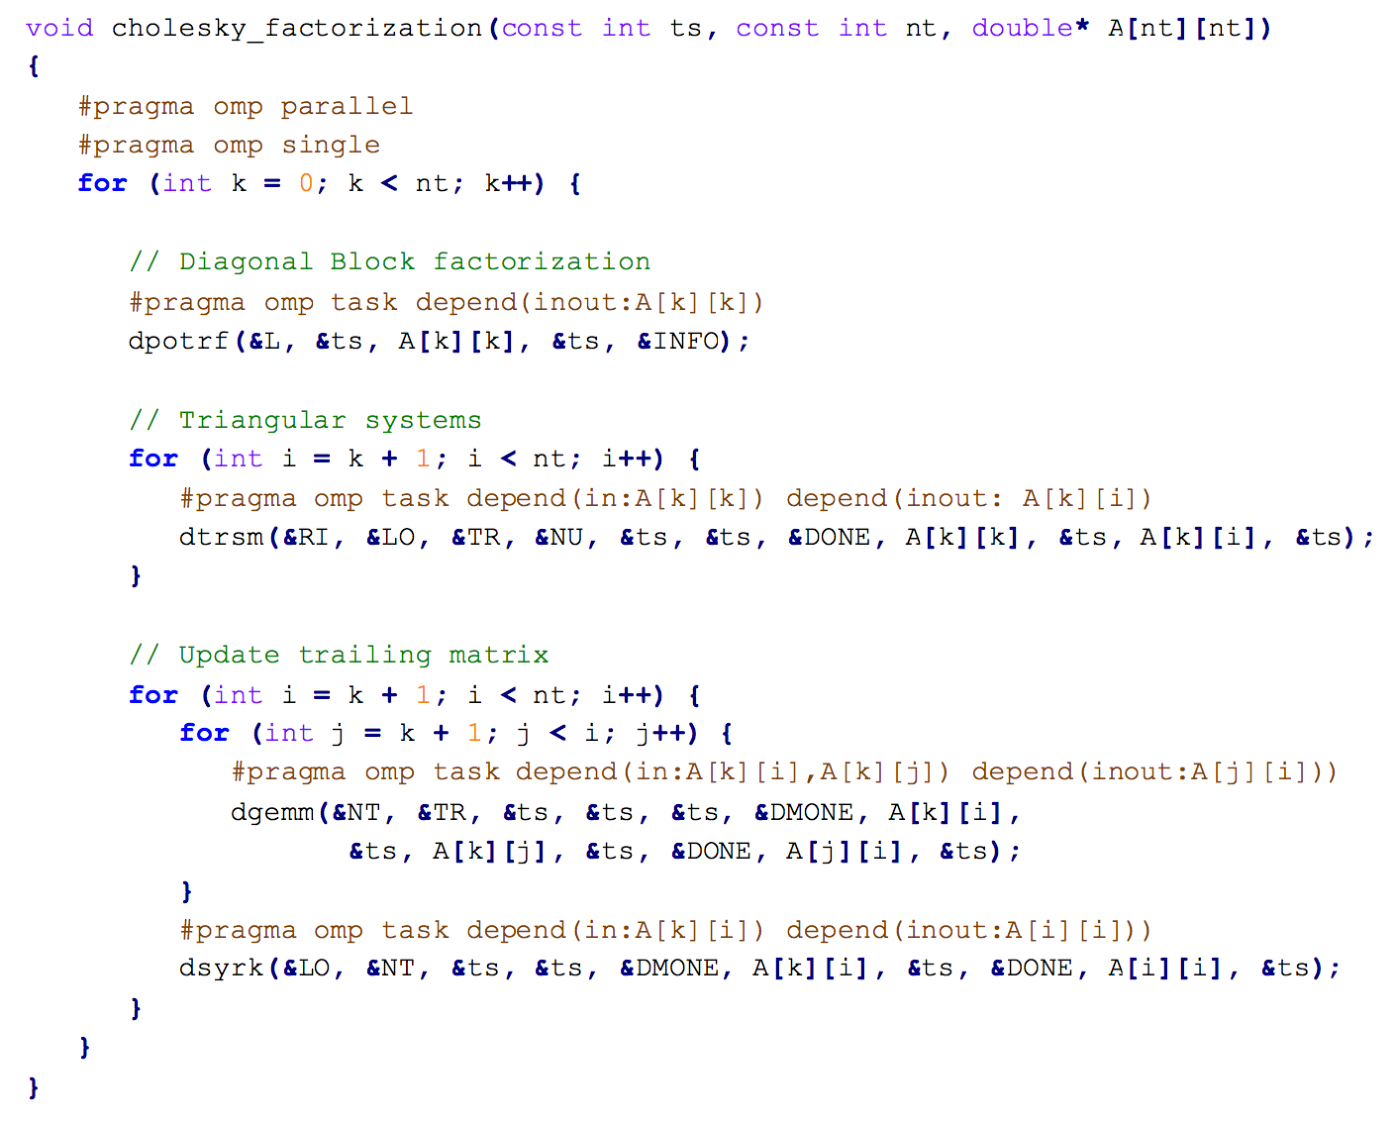
\includegraphics[width=0.85\textwidth]{images/cholesky}
      \caption{The Mixed Use of OpenMP Tasking and Intel MKL Library for Cholesky Factorization~\cite{intertwine}}
 \label{fig:cholesky}
\end{figure}


\subsubsection{Interacting with inter-node programming model, e.g. MPI}
Hybrid parallel programming in the form of internode+intranode, e.g. MPI+X model are widely used for 
for high-performance computing. This approach reflects the two-level hierarchy of parallelism in current HPC systems, 
in which a high-speed interconnect
joins many highly parallel nodes.
Interoperability between inter-node programming model such as MPI and OpenMP 
systems has long been a productivity and composability goal within
the parallel programming community. We however still have not agreed on a standard solution from either of the two communities. 




%\subsubsection{OpenMP with native threads}
%\subsubsection{OpenMP with TBB/MKL}
%\subsubsection{OpenMP with parallel scientific library, such as MKL}
%\subsubsection{Linking libraries and objects built with different OpenMP compilers}
%\subsubsection{OpenMP with inter-node model, e.g. MPI}


\subsection{Issues with Poor Interoperability}
\subsubsection{CPU Oversubscription}
Oversubscription happens when resources are claimed and held than what is needed.
A program may request more OpenMP threads than the total amount of hardware
threads available when entering a parallel region, which causes excessive competition 
among OpenMP threads for hardware threads and increases runtime overhead. 
When program execution enters into sequential stage after exiting a parallel region, 
those native threads that support the OpenMP threads in the parallel region may still 
alive in the background consuming CPU cycles. This 
will make those hardware threads unavailable to others. 
Oversubscription impact the performance of an applications and the system, 
but should not introduce correctness issue to a program. 

%A typical OpenMP runtime creates a pool of native threads who will execute OpenMP
% parallel regions and/or tasks. 

The two scenarios we mentioned above are the two kinds of oversubscription we should try to avoid:
{\bf 1) Active oversubscription}: Claiming or requesting more threads than 
what are available by the system.
{\bf 2) Passive oversubscription}: Thread resources are not released 
after parallel execution. Holding hardware threads after parallel execution may not 
always hurt the performance overall, e.g. it will improve the start-up performance of the 
upcoming parallel region. In this category, we are concerning those situations that 
actually impact the performance negatively.



\subsubsection{Conflicting Thread Affinity}
Besides oversubscribing computational resources (hardwre cores) by an OpenMP program, 
memory and thread affinity are another kinds of resources that should be coordinately allocated and managed among
multiple parallel runtimes. %about how resources are utilized. 
Thread affinity conflict happens when an OpenMP runtime binds threads data to 
certain memory places (cache or NUMA region) that are already occupied by 
the affinity requests of another runtime. Such overlaps cause excessive cache or memory spills or relocation of data
to further places, resulting increased memory access latency becasue of false sharing or 
poor locality of thread and its data. %the places.
The affinity conflicts can happen even the total number of threads requested does not exceed the number of hardware threads available.
%Obviously, conflicting thread affinity may adversely impact the performance of programs involved. 



\subsubsection{Global Impact of Environment Variables}
The interoperability and composability of OpenMP programs are also limited by the global impact of OpenMP environment variables.
Currently, the OpenMP specification has an implicit assumption that a single OpenMP program is running on a computation node at any given time.
So the provided global environment variables should work properly to set the internal control variables that affect the execution
of the single OpenMP program. 
However, this causes problem when multiple OpenMP programs are running simultaneously on a computation node. 
Environment variables affecting resource allocation may uniformly impact all OpenMP programs, which is often not desired.
For example, unless runtime library routines are explicitly used to customize each program's choices, \lstinline{OMP_NUM_THREADS}, \lstinline{OMP_PROC_BIND}, \lstinline{OMP_DEFAULT_DEVICE} may 
make all OpenMP runtime instances use the same number of threads, the same affinity, and the same accelerator device, respectively. 



\subsection{Limitation of Interoperability Support in the Standard}
OpenMP currently (4.0) provides limited support for users to give hints to runtime for 
better managing OpenMP threads and native threads, which can be used to help reducing 
the impact of oversubscriptions.
\paragraph{OMP\_DYNAMIC} % environment variable}
This also includes dynvar ICV, omp\_set\_dynamic and omp\_get\_dynamic runtime routine. OMP\_DYNAMIC could be either
{\bf true} or {\bf false}. When setting the dynvar ICV to be {\bf true}, user will expect
OpenMP implementation to adjust the number of threads to use for executing parallel
regions in order to optimize the use of system resources.

\paragraph{OMP\_WAIT\_POLICY} %environment variable}
This also include waitpolicyvar ICV, but no getter and setter routine. 
OMP\_WAIT\_POLICY could be set as either ACTIVE or PASSIVE. 
The ACTIVE value specifies that waiting threads should mostly be active, consuming processor
 cycles, while waiting. An OpenMP implementation may, for example, make waiting threads spin.
 The PASSIVE value specifies that waiting threads should mostly be passive, not consuming
 processor cycles, while waiting. For example, an OpenMP implementation may make waiting
 threads yield the processor to other threads or go to sleep.
 The details of the ACTIVE and PASSIVE behaviors are implementation defined.
 
 \paragraph{OMP\_THREAD\_LIMIT}
 This also include threadlimitvar ICV and omp\_get\_thread\_limit getter runtime routine.
 The environment variable sets the maximum number of OpenMP threads to use in a contention group by setting the threadlimitvar ICV.
The behavior of the program is implementation defined if the requested value of OMP\_THREAD\_LIMIT is greater than the number of threads an implementation can support

OMP\_DYNAMIC and OMP\_THREAD\_LIMIT are approaches to
addressing active oversubscriptions, and OMP\_WAIT\_POLICY could be used to address
passive oversubscriptions. 
Since there are no setters for ICVs for OMP\_WAIT\_POLICY
and OMP\_THREAD\_LIMIT variable in the current standard, 
dynamically changing waiting policy and the maximum number of
threads at runtime is not available.
